% !TeX program = xelatex
% !TeX options = -shell-escape -synctex=1 -interaction=nonstopmode -file-line-error "%DOC%"
\documentclass[aspectratio=169,11pt]{beamer}

% ———- голый beamer: никаких полос, тем и навигации ———-
\setbeamertemplate{navigation symbols}{}
\setbeamertemplate{headline}{}
\setbeamertemplate{footline}{}
\setbeamertemplate{frametitle}{}
\setbeamersize{text margin left=0pt, text margin right=0pt}

\usepackage{fontspec}
\setmainfont{Inter}[Ligatures=TeX]
\setsansfont{Inter}[Ligatures=TeX]
\newfontfamily\InterBold{Inter Bold}[Ligatures=TeX]
\newfontfamily\InterSemi{Inter SemiBold}[Ligatures=TeX]

\usepackage{tikz}
\usetikzlibrary{arrows.meta,positioning,calc,shadows.blur}
\usepackage{graphicx}
\usepackage{booktabs}
\usepackage{array}
\usepackage{colortbl}
\usepackage{hhline}
\usepackage{tabularx}

\newcolumntype{L}[1]{>{\raggedright\arraybackslash}m{#1}}
\newcolumntype{C}[1]{>{\centering\arraybackslash}m{#1}}

% ———- палитра М.Видео ———-
\definecolor{mvred}{HTML}{E30613}
\definecolor{mvdark}{HTML}{1C1C1E}
\definecolor{mvgray}{HTML}{6E6E73}
\definecolor{cardbg}{HTML}{F5F5F6}
\definecolor{pinkband}{HTML}{FDECEC}
\definecolor{okgreen}{HTML}{1F8A50}
\definecolor{warnorange}{HTML}{C75000}
\definecolor{mvborder}{HTML}{E3D8D8}

\graphicspath{{assets/}{../figures/}{../figures/apps/}{figures/}{../figures/gliner/}{../figures/general_study/}{../figures/complex_eda/}{../figures/brand_clf/}{preview/day4/}}

% ———- макро ———-
\newcommand{\kicker}[1]{{\color{mvred}\InterBold\fontsize{8}{10}\selectfont\MakeUppercase{#1}}}
\newcommand{\slidetitle}[1]{{\color{mvdark}\InterBold\fontsize{15.5}{18}\selectfont #1}}

\newcommand{\pinknote}[2]{%
  \begin{tikzpicture}
    \node[fill=pinkband, rounded corners=2pt, inner xsep=9pt, inner ysep=5.5pt,
          text width=\dimexpr\textwidth-18pt\relax] {%
      {\color{mvred}\InterBold\fontsize{8}{10}\selectfont #1}\hspace{7pt}{\color{mvdark}\fontsize{8.5}{11}\selectfont #2}};
  \end{tikzpicture}}
\newcommand{\conclusion}[1]{\pinknote{ВЫВОД}{#1}}

\newcommand{\graynote}[2]{%
  \begin{tikzpicture}
    \node[fill=cardbg, rounded corners=2pt, inner xsep=9pt, inner ysep=5.5pt,
          text width=\dimexpr\textwidth-18pt\relax] {%
      {\color{mvdark}\InterBold\fontsize{8}{10}\selectfont #1}\hspace{7pt}{\color{mvdark}\fontsize{8.5}{11}\selectfont #2}};
  \end{tikzpicture}}

\newcommand{\numdot}[1]{%
  \tikz[baseline=-0.6ex]{\node[circle, fill=mvred, text=white, inner sep=1pt, minimum size=12pt, font=\InterBold\fontsize{7}{8}\selectfont]{#1};}}

\newcommand{\cornerlogo}{%
  \begin{tikzpicture}[remember picture, overlay]
    \node[anchor=north east, xshift=-0.5cm, yshift=-0.38cm] at (current page.north east)
      {
\includegraphics[height=0.85cm]{m_letter.png}};
  \end{tikzpicture}}

\newcommand{\slidehead}[2]{%
  \cornerlogo
  \vspace{0.38cm}\par
  \hspace{0.85cm}\begin{minipage}{\dimexpr\paperwidth-1.7cm\relax}
  \kicker{#1}\par\vspace{3pt}
  \slidetitle{#2}\par\vspace{7pt}}
\newcommand{\slidefoot}{\end{minipage}}

\newcommand{\bodytext}{\fontsize{8.5}{11.5}\selectfont}
\newcommand{\smalltext}{\fontsize{7.5}{10}\selectfont}

\definecolor{tblline}{HTML}{DDDDDD}
\arrayrulecolor{tblline}
\newcommand{\ttext}{\fontsize{7}{9}\selectfont}
\newcommand{\thead}[1]{\cellcolor{mvdark}{\color{white}\InterSemi\ttext #1}}
\newcommand{\theadl}[1]{\cellcolor{mvdark}{\color{white}\InterSemi\ttext #1}}
\newcommand{\tacc}[1]{\cellcolor{mvred}{\color{white}\InterSemi\ttext #1}}
\newcommand{\tcellc}[1]{{\ttext\color{mvdark}#1}}
\newcommand{\tcelll}[1]{{\ttext\color{mvdark}#1}}
\newcommand{\hnum}[1]{{\InterBold\color{mvdark}#1}}
\newcommand{\hb}[1]{{\InterSemi\color{mvdark}#1}}
\newcommand{\tnote}[1]{{\color{mvred}\itshape\fontsize{7}{9}\selectfont #1}}

\newcommand{\wtag}[2]{\tikz[baseline=-0.55ex]{\node[rounded corners=2pt, fill=#1, inner xsep=4pt, inner ysep=2.2pt, font=\InterSemi\fontsize{7.8}{9}\selectfont, text=white]{#2};}}
\newcommand{\wplain}[1]{\tikz[baseline=-0.55ex]{\node[rounded corners=2pt, fill=cardbg, inner xsep=4pt, inner ysep=2.2pt, font=\fontsize{7.8}{9}\selectfont, text=mvdark]{#1};}}

\newcommand{\chevron}{%
  \raisebox{-0.15ex}{\begin{tikzpicture}
    \draw[mvred, line width=1.3pt, line cap=round, line join=round]
      (0,0.13) -- (0.065,0.065) -- (0,0);
  \end{tikzpicture}}}
\newcommand{\pipestep}[3]{%
  \begin{tikzpicture}[baseline=(b.center)]
    \node[fill=#1, rounded corners=3pt, minimum height=0.92cm, text width=1.72cm,
          align=center, inner sep=2.5pt, font=\InterSemi\fontsize{6.6}{8}\selectfont, text=#2] (b) {#3};
  \end{tikzpicture}}
\newcommand{\pipestepw}[3]{%
  \begin{tikzpicture}[baseline=(b.center)]
    \node[fill=#1, rounded corners=3pt, minimum height=0.92cm, text width=2.05cm,
          align=center, inner sep=2.5pt, font=\InterSemi\fontsize{6.6}{8}\selectfont, text=#2] (b) {#3};
  \end{tikzpicture}}
\newcommand{\iconcard}[3]{%
  \begin{tikzpicture}
    \node[fill=cardbg, rounded corners=4pt, inner sep=6pt, text width=3.05cm, align=center,
          minimum height=2.05cm, anchor=north] (c) {%
      {\InterSemi\fontsize{8}{10}\selectfont\color{mvdark}#1}\par\vspace{3pt}
      {\fontsize{6.6}{8.4}\selectfont\color{mvgray}#2#3}};
  \end{tikzpicture}}
\newcommand{\agendaitem}[3]{%
  \begin{tikzpicture}
    \node[fill=cardbg, rounded corners=4pt, inner sep=7pt, text width=3.7cm, align=left,
          minimum height=1.55cm] {%
      {\color{mvred}\InterBold\fontsize{9}{11}\selectfont #1}\par\vspace{2pt}
      {\InterSemi\fontsize{8}{10}\selectfont\color{mvdark}#2}\par\vspace{1pt}
      {\fontsize{6.8}{8.5}\selectfont\color{mvgray}#3}};
  \end{tikzpicture}}

\setlength{\parskip}{0pt}

\begin{document}

% ============================================================
% 1. ТИТУЛ
% ============================================================
\begin{frame}[plain]
\begin{tikzpicture}[remember picture, overlay]
  \fill[mvred] (current page.south west) rectangle (current page.north east);
  \node[anchor=east, inner sep=0pt] at ([xshift=0.32\paperwidth]current page.east)
    {
\includegraphics[height=1.06\paperheight]{kurs1_image1.png}};
  \node[anchor=west, align=left] at ([xshift=0.9cm, yshift=2.15cm]current page.west)
    {\color{white}\InterBold\fontsize{10}{12}\selectfont БУТКЕМП М.ВИДЕО · NLP / SEARCH · ИТОГИ};
  \node[anchor=west, align=left] at ([xshift=0.88cm, yshift=0.95cm]current page.west)
    {\color{white}\InterBold\fontsize{26}{30}\selectfont Умный поиск:};
  \node[anchor=west, align=left] at ([xshift=0.88cm, yshift=0.05cm]current page.west)
    {\color{white}\InterBold\fontsize{26}{30}\selectfont от данных до каскада};
  \node[anchor=west, align=left, text width=0.52\paperwidth] at ([xshift=0.9cm, yshift=-1.85cm]current page.west)
    {\color{white}\fontsize{11}{15}\selectfont Query Understanding для М.Видео: EDA $\to$ MVP-каскад $\to$ SpellFix, GLiNER и честные метрики на золоте.};
  \node[anchor=south west] at ([xshift=0.9cm, yshift=0.5cm]current page.south west)
    {\color{white}\fontsize{9}{11}\selectfont Итоговая презентация · Дни 02--04};
\end{tikzpicture}
\end{frame}

% ============================================================
% 2. АГЕНДА
% ============================================================
\begin{frame}[t]
\slidehead{структура}{О чём расскажем}
\vspace{4pt}\par
\begin{center}
\begin{tikzpicture}[node distance=10pt]
  \node (a1) {\agendaitem{01}{Задача и данные}{масштаб, короткие запросы,\\главный инсайт EDA}};
  \node[right=of a1] (a2) {\agendaitem{02}{Пайплайн}{гибридный каскад\\и что реально в проде}};
  \node[right=of a2] (a3) {\agendaitem{03}{День 04}{SpellFix, журнал,\\GLiNER, joint study}};
\end{tikzpicture}
\par\vspace{10pt}
\begin{tikzpicture}[node distance=10pt]
  \node (b1) {\agendaitem{04}{Метрики}{gold vs silver,\\что работает на опечатках}};
  \node[right=of b1] (b2) {\agendaitem{05}{Честно}{ограничения и\\следующие шаги}};
  \node[right=of b2] (b3) {\agendaitem{06}{Демо}{поиск и разметка\\как продукт}};
\end{tikzpicture}
\end{center}
\slidefoot
\end{frame}

% ============================================================
% 3. ЗАДАЧА
% ============================================================
\begin{frame}[t]
\slidehead{задача}{Не «ещё один NER», а понимание запроса}
\pinknote{ЦЕЛЬ}{Из короткой строки пользователя достать факты (бренд, категория, модель, атрибуты) и отдать их поиску / фильтрам — быстро, интерпретируемо, с запасными слоями.}
\vspace{8pt}\par
\begin{columns}[T]
\column{0.48\textwidth}
{\InterSemi\fontsize{8.5}{10.5}\selectfont Почему сложно}\par\vspace{5pt}
{\smalltext
\numdot{1}\ Запросы короткие: 1--3 токена, часто без бренда.\par\vspace{4pt}
\numdot{2}\ Опечатки, смесь кириллицы/латиницы, транслит.\par\vspace{4pt}
\numdot{3}\ Клики шумные: кликнули не то, что написали.\par\vspace{4pt}
\numdot{4}\ Одна модель на всём не закрывает SLA и edge-cases.}
\column{0.48\textwidth}
{\InterSemi\fontsize{8.5}{10.5}\selectfont Наш ответ}\par\vspace{5pt}
{\smalltext
\numdot{1}\ \textbf{Словари и правила} — мгновенный слой.\par\vspace{4pt}
\numdot{2}\ \textbf{CRF} — морфология и контекст токенов.\par\vspace{4pt}
\numdot{3}\ \textbf{Классификаторы} — скрытый бренд и тип ATTR.\par\vspace{4pt}
\numdot{4}\ \textbf{SpellFix} — чиним текст \emph{до} моделей.\par\vspace{4pt}
\numdot{5}\ \textbf{GLiNER} — гибкий хвост (пока эксперимент).}
\end{columns}
\slidefoot
\end{frame}

% ============================================================
% 4. ДАННЫЕ (из дня 2)
% ============================================================
\begin{frame}[t]
\slidehead{день 02 · данные}{С чем работаем}
\conclusion{Данных достаточно и для словарей, и для обучения: узкое место не объём, а качество меток.}
\vspace{8pt}\par
\begin{columns}[T]
\column{0.31\textwidth}
{\color{mvred}\InterBold\fontsize{13.5}{15.5}\selectfont 30.99 млн}\par
{\smalltext\color{mvgray} кликов: запрос $\to$ SKU}
\vspace{6pt}\par
{\color{mvred}\InterBold\fontsize{13.5}{15.5}\selectfont 1.79 млн}\par
{\smalltext\color{mvgray} уникальных запросов}
\vspace{6pt}\par
{\color{mvred}\InterBold\fontsize{13.5}{15.5}\selectfont 1.18 млн}\par
{\smalltext\color{mvgray} карточек title + description}
\column{0.31\textwidth}
{\color{mvred}\InterBold\fontsize{13.5}{15.5}\selectfont 333 тыс}\par
{\smalltext\color{mvgray} уникальных SKU в кликах}
\vspace{6pt}\par
{\color{mvred}\InterBold\fontsize{13.5}{15.5}\selectfont 7 150}\par
{\smalltext\color{mvgray} брендов}
\vspace{6pt}\par
{\color{mvred}\InterBold\fontsize{13.5}{15.5}\selectfont 546 тыс}\par
{\smalltext\color{mvgray} офферов в YML-каталоге}
\column{0.34\textwidth}
\begin{tikzpicture}
\node[fill=cardbg, rounded corners=3pt, inner sep=7pt, text width=\dimexpr\textwidth-14pt\relax]{
{\InterSemi\fontsize{8}{10}\selectfont Пример строки клика}\par\vspace{4pt}
{\fontsize{7}{9}\selectfont\color{mvgray}
query: «galaxy s25»\par
sku: Смартфон Samsung Galaxy S25 FE 8/256GB Black\par
brand: Samsung · price: 50 703 ₽ · position: 2}
};
\end{tikzpicture}
\end{columns}
\slidefoot
\end{frame}

% ============================================================
% 5. КЛЮЧЕВОЙ ИНСАЙТ ДНЯ 2
% ============================================================
\begin{frame}[t]
\slidehead{день 02 · ключевой инсайт}{73\% брендов нет в тексте запроса}
\begin{columns}[T]
\column{0.44\textwidth}
\vspace{2pt}\centering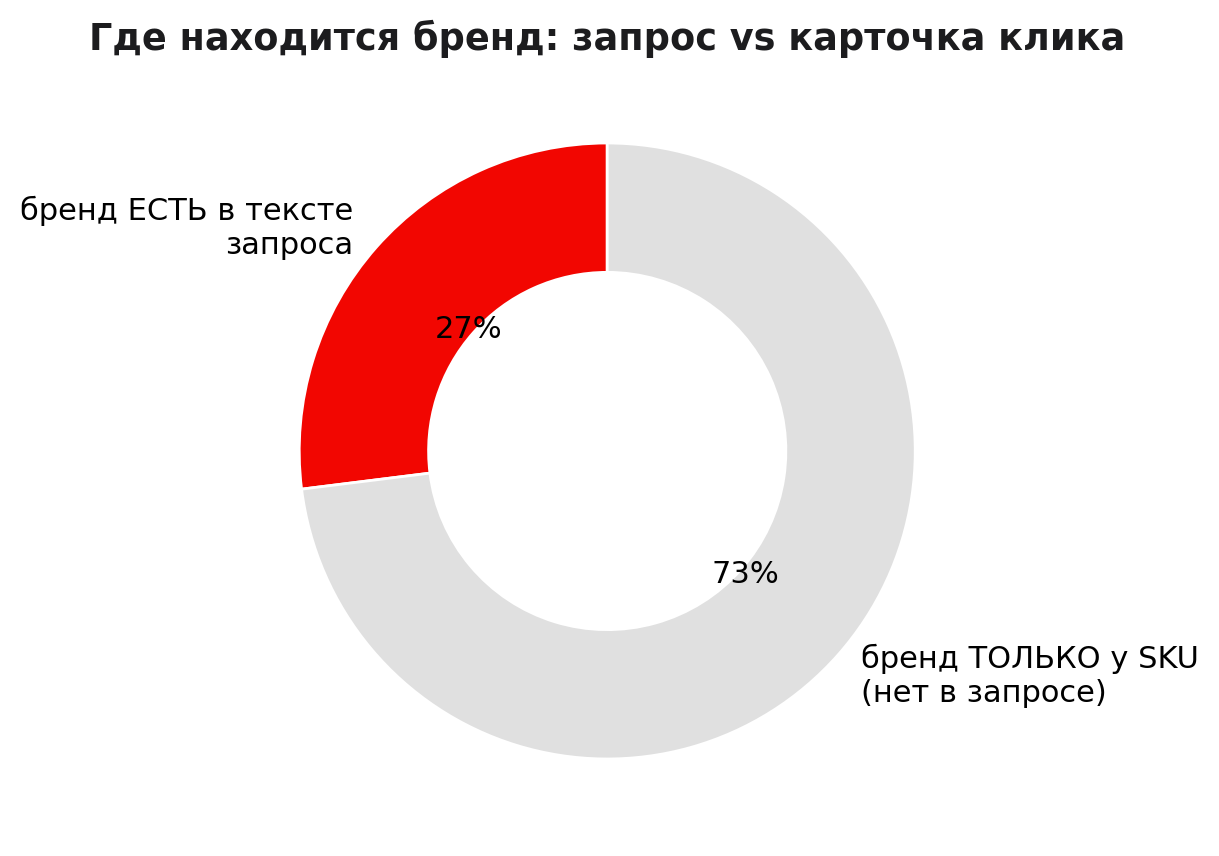
\includegraphics[width=0.98\textwidth]{eda_brand_in_query.png}
\column{0.53\textwidth}
\conclusion{Только в \textbf{27\%} кликов бренд написан в запросе. Поэтому в каскаде нужен не только словарь, но и классификатор бренда.}
\vspace{6pt}\par
{\smalltext
\numdot{1}\ Голова трафика — категорийные запросы без бренда.\par\vspace{4pt}
\numdot{2}\ Клики живут в топе выдачи — шум смешивается с сигналом.\par\vspace{4pt}
\numdot{3}\ Отсюда архитектура: правила $\to$ NER $\to$ запасной бренд-слой.}
\end{columns}
\slidefoot
\end{frame}

% ============================================================
% 6. ПАЙПЛАЙН СЕГОДНЯ
% ============================================================
\begin{frame}[t]
\slidehead{пайплайн · прод}{Гибридный каскад, который работает сейчас}
\pinknote{В ПРОДЕ}{\texttt{SpellFix $\to$ правила/словари $\to$ CRF $\to$ brand\_clf $\to$ типизатор ATTR}. Тот же каскад в Qt .exe, FastAPI и CLI. GLiNER обучен и измерен, в сервис пока не вшит.}
\vspace{8pt}\par
\begin{center}
\begin{tikzpicture}[node distance=0pt]
  \node (a) {\pipestep{cardbg}{mvdark}{ЗАПРОС\\\fontsize{5.4}{6.4}\selectfont «телфон 16гь»}};
  \node[right=1pt of a] (c1) {\chevron};
  \node[right=1pt of c1] (b) {\pipestep{mvred}{white}{SPELLFIX\\\fontsize{5.4}{6.4}\selectfont опечатки}};
  \node[right=1pt of b] (c2) {\chevron};
  \node[right=1pt of c2] (d) {\pipestep{cardbg}{mvdark}{ПРАВИЛА\\\fontsize{5.4}{6.4}\selectfont словари}};
  \node[right=1pt of d] (c3) {\chevron};
  \node[right=1pt of c3] (e) {\pipestep{cardbg}{mvdark}{CRF\\\fontsize{5.4}{6.4}\selectfont BIO-теги}};
  \node[right=1pt of e] (c4) {\chevron};
  \node[right=1pt of c4] (f) {\pipestep{cardbg}{mvdark}{BRAND\\\fontsize{5.4}{6.4}\selectfont классиф.}};
  \node[right=1pt of f] (c5) {\chevron};
  \node[right=1pt of c5] (g) {\pipestep{mvdark}{white}{ATTR\\\fontsize{5.4}{6.4}\selectfont марков}};
\end{tikzpicture}
\end{center}
\vspace{10pt}\par
{\smalltext
\numdot{1}\ Каждый слой закрывает слабость предыдущего: словарь — мгновенно, CRF — морфологию, brand\_clf — скрытый бренд.\par\vspace{4pt}
\numdot{2}\ Одинаковый SpellFix и при сборке silver, и в бою — модель не видит «грязный» текст только в проде.\par\vspace{4pt}
\numdot{3}\ На выходе — структурированные факты (entities + attributes), а не «чёрный ящик».}
\slidefoot
\end{frame}

% ============================================================
% 7. MVP ДНЯ 3 — ПРОДУКТ
% ============================================================
\begin{frame}[t]
\slidehead{день 03 · mvp}{Что собрали как продукт}
\vspace{2pt}\par
\begin{center}
\begin{tikzpicture}[node distance=10pt]
  \node (o1) {\iconcard{Предобработка}{единый слой очистки\\}{запроса до моделей}};
  \node[right=of o1] (o2) {\iconcard{Тег MODEL}{майнинг словаря\\}{моделей из кликов}};
  \node[right=of o2] (o3) {\iconcard{Каскад моделей}{CRF + brand\_clf\\}{+ типизатор ATTR}};
  \node[right=of o3] (o4) {\iconcard{Два приложения}{умный поиск\\}{и разметка BIO}};
\end{tikzpicture}
\end{center}
\vspace{8pt}\par
\begin{columns}[T]
\column{0.48\textwidth}
{\InterSemi\fontsize{8.5}{10.5}\selectfont Brand classifier}\par\vspace{4pt}
{\smalltext 67 классов, в т.ч. NO\_BRAND / UNKNOWN · macro-F1 $\approx$ \textbf{0{,}94} на silver-val · лучше отказать, чем подставить ложный бренд.}
\column{0.48\textwidth}
{\InterSemi\fontsize{8.5}{10.5}\selectfont CRF + ATTR}\par\vspace{4pt}
{\smalltext CRF на слабой BIO-разметке · марковский типизатор атрибутов рядом с правилами · петля качества через ручную разметку.}
\end{columns}
\slidefoot
\end{frame}

% ============================================================
% 7b. FASTAPI + CLI
% ============================================================
\begin{frame}[t]
\slidehead{сервис · fastapi}{HTTP API и CLI для того же каскада}
\pinknote{ОДИН EXTRACTOR}{Настольный Qt-движок, FastAPI и CLI ходят в одну логику фактов: SpellFix $\to$ правила $\to$ CRF $\to$ brand/ATTR. Меняем слой один раз — проверяем тремя способами.}
\vspace{6pt}\par
\begin{columns}[T]
\column{0.48\textwidth}
{\InterSemi\fontsize{8.5}{10.5}\selectfont FastAPI (\texttt{src/service})}\par\vspace{4pt}
{\smalltext
\numdot{1}\ \texttt{POST /extract} — JSON фактов для интеграции.\par\vspace{3pt}
\numdot{2}\ \texttt{POST /extract/debug} — BIO-пайплайны для лаборатории.\par\vspace{3pt}
\numdot{3}\ \texttt{GET /health} — готовность моделей и словарей.\par\vspace{3pt}
\numdot{4}\ Веб-UI из \texttt{web/} на том же порту.}
\column{0.48\textwidth}
{\InterSemi\fontsize{8.5}{10.5}\selectfont CLI + журнал}\par\vspace{4pt}
{\smalltext
\numdot{1}\ \texttt{python -m src.cli.cli "запрос"} — быстрый smoke-тест каскада.\par\vspace{3pt}
\numdot{2}\ Режим \texttt{-i} / \texttt{--demo} для демо без UI.\par\vspace{3pt}
\numdot{3}\ \texttt{artifacts/history/} — снимки метрик CRF/brand/ATTR и broken queries (не теряются в git-диффах).}
\end{columns}
\slidefoot
\end{frame}

% ============================================================
% 8. ДЕНЬ 4 — ЧТО ДОБАВИЛИ
% ============================================================
\begin{frame}[t]
\slidehead{день 04 · новшества}{Что изменилось после MVP}
\pinknote{КОРОТКО}{Закрыли шум на входе, завели человекочитаемый журнал экспериментов, прогнали GLiNER как хвост и впервые измерили весь каскад на трёх типах данных.}
\vspace{8pt}\par
\begin{center}
\begin{tikzpicture}[node distance=10pt]
  \node (o1) {\iconcard{SpellFix v2}{гомоглифы, fuzzy,\\}{алиасы транслита}};
  \node[right=of o1] (o2) {\iconcard{CRF rebuild}{пересборка silver\\}{+ gold microF1 $\uparrow$}};
  \node[right=of o2] (o3) {\iconcard{Журнал}{\texttt{artifacts/history}\\}{метрики + кейсы}};
  \node[right=of o3] (o4) {\iconcard{GLiNER + joint}{один silver,\\}{метрика пайплайна}};
\end{tikzpicture}
\end{center}
\slidefoot
\end{frame}

% ============================================================
% 9. SPELLFIX
% ============================================================
\begin{frame}[t]
\slidehead{spellfix v2}{Опечатки, гомоглифы и транслит — до модели}
\begin{columns}[T]
\column{0.52\textwidth}
{\InterSemi\fontsize{8.5}{10.5}\selectfont Три механики}\par\vspace{5pt}
{\renewcommand{\arraystretch}{1.3}\setlength{\tabcolsep}{5pt}
\begin{tabular}{|L{2.5cm}|L{4.0cm}|}
\hline
\theadl{Механика} & \theadl{Пример}\\
\hline
\tcelll{\hb{Fuzzy + клавиатура}} & \tcelll{«16гь» $\to$ «16 гб», «телфон» $\to$ «телефон»}\\
\hline
\tcelll{\hb{Гомоглифы}} & \tcelll{кир./лат. двойники: c/с, a/а, e/е}\\
\hline
\tcelll{\hb{Алиасы}} & \tcelll{«сони» $\to$ «sony», «ксяоми» $\to$ «xiaomi»}\\
\hline
\end{tabular}}
\column{0.44\textwidth}
{\InterSemi\fontsize{8.5}{10.5}\selectfont Эффект на CRF}\par\vspace{5pt}
{\smalltext
SpellFix тронул \textbf{767 / 5000} silver-запросов до обучения.\par\vspace{5pt}
Gold micro-F1: \textbf{0{,}582 $\to$ 0{,}594}.\par\vspace{5pt}
Сильнее всего вырос ATTR (+0{,}07) — единицы с опечаткой больше не ломают учителя.}
\end{columns}
\vspace{6pt}\par
\conclusion{Одна функция чинит текст и при сборке обучающих данных, и в бою — без отдельного «продакшен-режима».}
\slidefoot
\end{frame}

% ============================================================
% 10. BROKEN QUERIES + ЖУРНАЛ
% ============================================================
\begin{frame}[t]
\slidehead{день 04 · журнал}{Честные кейсы и история экспериментов}
\begin{columns}[T]
\column{0.52\textwidth}
{\InterSemi\fontsize{8.5}{10.5}\selectfont SpellFix справляется}\par\vspace{4pt}
{\smalltext\color{mvgray}
\wplain{телфон 16 гь} \chevron\ \wplain{телефон 16 гб}\par\vspace{3pt}
\wplain{планше тxiaomi} \chevron\ \wplain{планшет xiaomi}\par\vspace{3pt}
\wplain{ноутбок asus 16гь} \chevron\ \wplain{ноутбук asus 16 гб}}
\par\vspace{7pt}
{\InterSemi\fontsize{8.5}{10.5}\selectfont Пока нет}\par\vspace{4pt}
{\smalltext\color{mvgray}
\wplain{моильник 16 гб} — слишком далёкая порча (3 буквы), вне fuzzy}
\column{0.44\textwidth}
\graynote{HISTORY}{\texttt{artifacts/history/} — снимки метрик CRF / brand / ATTR + \texttt{broken\_queries.md}. Git хранит код; сюда пишем «что поменяли и что получили».}
\vspace{6pt}\par
\pinknote{НЕ СПРЯТАЛИ}{На «sony ps5» NER ок, но \texttt{category\_clf} иногда путает PlayStation с феном/смартфоном — отдельный баг, не SpellFix.}
\end{columns}
\slidefoot
\end{frame}

% ============================================================
% 11. GLINER ZERO-SHOT
% ============================================================
\begin{frame}[t]
\slidehead{gliner · zero-shot}{Что даёт модель без дообучения}
\begin{columns}[T]
\column{0.46\textwidth}
\vspace{2pt}\centering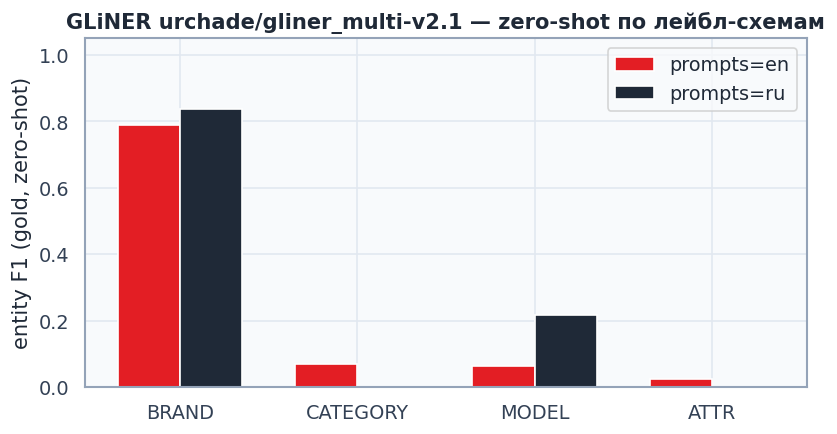
\includegraphics[width=0.95\textwidth,height=4.7cm,keepaspectratio]{01_zero_shot_f1.png}
\column{0.5\textwidth}
\graynote{МОДЕЛЬ}{\texttt{urchade/gliner\_multi-v2.1} — мультиязычный чекпоинт. Роль — гибкий хвост, не замена CRF.}
\vspace{5pt}\par
{\smalltext
\numdot{1}\ Лучшая схема промпта — английские лейблы: micro-F1 \textbf{0{,}35} на gold.\par\vspace{4pt}
\numdot{2}\ BRAND находится и без обучения (F1 $\approx$0{,}79).\par\vspace{4pt}
\numdot{3}\ CATEGORY / ATTR почти пустые — домену нужны примеры.}
\end{columns}
\slidefoot
\end{frame}

% ============================================================
% 12. GLINER FINE-TUNE
% ============================================================
\begin{frame}[t]
\slidehead{gliner · fine-tune}{После обучения на gold + silver}
\begin{columns}[T]
\column{0.46\textwidth}
\vspace{2pt}\centering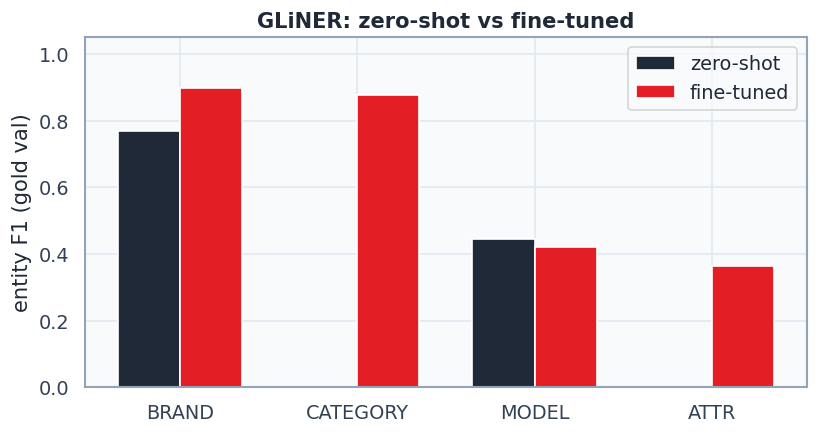
\includegraphics[width=0.95\textwidth,height=4.7cm,keepaspectratio]{02_finetune_f1.png}
\column{0.5\textwidth}
\conclusion{micro-F1 \textbf{0{,}39 $\to$ 0{,}74}: CATEGORY подтянулась с 0 до 0{,}88 — модель увидела домен.}
\vspace{5pt}\par
{\smalltext
\numdot{1}\ Порог откалиброван отдельно ($\approx$0{,}35): default 0{,}5 резал верные, но неуверенные спаны.\par\vspace{4pt}
\numdot{2}\ ATTR остаётся самым слабым (F1 $\approx$0{,}36) — мало и шумно в gold.\par\vspace{4pt}
\numdot{3}\ В прод не подключён: сначала гейт и latency-бюджет.}
\end{columns}
\slidefoot
\end{frame}

% ============================================================
% 13. JOINT STUDY
% ============================================================
\begin{frame}[t]
\slidehead{joint study}{Один silver — честное сравнение каскада}
\pinknote{ИДЕЯ}{CRF и GLiNER на \textbf{одном} silver; gold — held-out. Стадии: rules $\to$ +CRF $\to$ +GLiNER.}
\vspace{3pt}\par
\begin{columns}[T]
\column{0.52\textwidth}
\vspace{1pt}\centering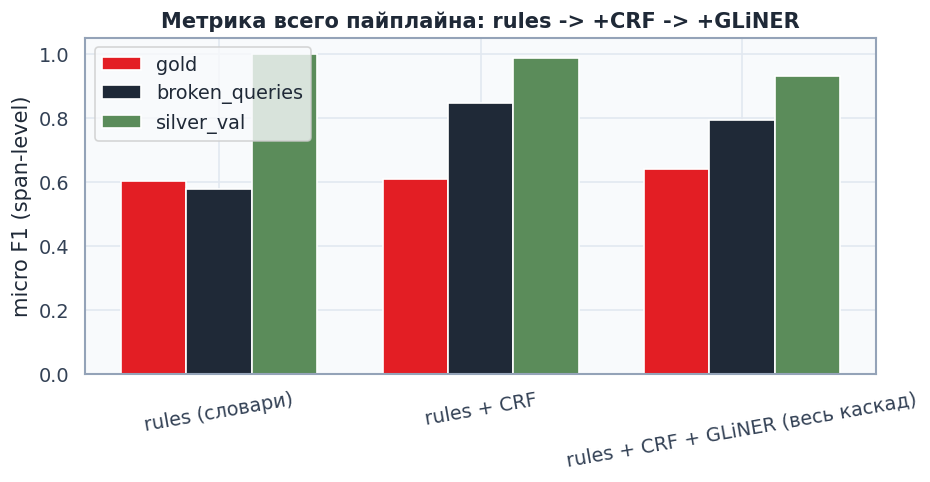
\includegraphics[width=0.98\textwidth,height=4.6cm,keepaspectratio]{02_pipeline_f1.png}
\column{0.44\textwidth}
{\smalltext
\numdot{1}\ На \textbf{broken} главный прирост — CRF: \textbf{0{,}58 $\to$ 0{,}85}.\par\vspace{3pt}
\numdot{2}\ На \textbf{gold} GLiNER сверху: \textbf{0{,}61 $\to$ 0{,}64}.\par\vspace{3pt}
\numdot{3}\ На шуме «слепой» хвост \textbf{портит} precision (0{,}85$\to$0{,}80).\par\vspace{3pt}
\numdot{4}\ Silver-val $\approx$1{,}0 — самосогласие teacher, не истина.}
\end{columns}
\vspace{2pt}\par
\conclusion{GLiNER звать только когда rules+CRF ничего не нашли — не для безусловного дозаполнения.}
\slidefoot
\end{frame}

% ============================================================
% 14. СВОДКА МЕТРИК
% ============================================================
\begin{frame}[t]
\slidehead{метрики · сводка}{Честные ориентиры на одной странице}
{\renewcommand{\arraystretch}{1.28}\setlength{\tabcolsep}{5pt}
\begin{tabular}{|L{4.2cm}|C{2.4cm}|C{2.4cm}|L{3.6cm}|}
\hline
\theadl{Что} & \thead{было} & \thead{стало} & \theadl{где смотреть}\\
\hline
\tcelll{CRF gold micro-F1} & \tcellc{0{,}582} & \tcellc{\hnum{0{,}594}} & \tcelll{после SpellFix}\\
\hline
\tcelll{Brand clf macro-F1} & \tcellc{—} & \tcellc{\hnum{0{,}94}} & \tcelll{silver-val}\\
\hline
\tcelll{Каскад gold (rules+CRF+GL)} & \tcellc{0{,}604} & \tcellc{\hnum{0{,}640}} & \tcelll{joint study}\\
\hline
\tcelll{Каскад broken (rules+CRF)} & \tcellc{0{,}578} & \tcellc{\hnum{0{,}846}} & \tcelll{устойчивость к шуму}\\
\hline
\tcelll{GLiNER FT gold} & \tcellc{0{,}39} & \tcellc{\hnum{0{,}74}} & \tcelll{изолированный трек}\\
\hline
\end{tabular}}
\vspace{8pt}\par
\tnote{Главное правило: silver-val красивый, но завышен. Решения принимаем по gold и по broken-кейсам.}
\slidefoot
\end{frame}

% ============================================================
% 15. ОГРАНИЧЕНИЯ + ДАЛЬШЕ
% ============================================================
\begin{frame}[t]
\slidehead{честно · дальше}{Что знаем и куда идём}
\begin{columns}[T]
\column{0.48\textwidth}
{\InterSemi\fontsize{8.5}{10.5}\selectfont Ограничения}\par\vspace{5pt}
{\smalltext
\numdot{1}\ Gold маленький (181) — хвостовые теги шумные.\par\vspace{4pt}
\numdot{2}\ GLiNER ещё не в \texttt{extractor.py}.\par\vspace{4pt}
\numdot{3}\ \texttt{category\_clf} ошибается на редких категориях.\par\vspace{4pt}
\numdot{4}\ Жёсткие порчи вроде «моильник» SpellFix не ловит.}
\column{0.48\textwidth}
{\InterSemi\fontsize{8.5}{10.5}\selectfont Следующие шаги}\par\vspace{5pt}
{\smalltext
\numdot{1}\ Расширить и дочистить gold $\to$ CRF v2.\par\vspace{4pt}
\numdot{2}\ Вшить GLiNER с гейтом (только пустые ответы).\par\vspace{4pt}
\numdot{3}\ Починить category\_clf на консолях/редких категориях.\par\vspace{4pt}
\numdot{4}\ Пополнять \texttt{spell\_aliases.txt} из разметки.}
\end{columns}
\vspace{8pt}\par
\conclusion{Пайплайн уже измерен на трёх типах данных — дальше усиливаем то, что реально работает, а не гонимся за красивым числом на silver.}
\slidefoot
\end{frame}

% ============================================================
% 16. ДЕМО / ПРИЛОЖЕНИЯ
% ============================================================
\begin{frame}[t]
\slidehead{продукт}{Два приложения команды}
\begin{columns}[T]
\column{0.48\textwidth}
\centering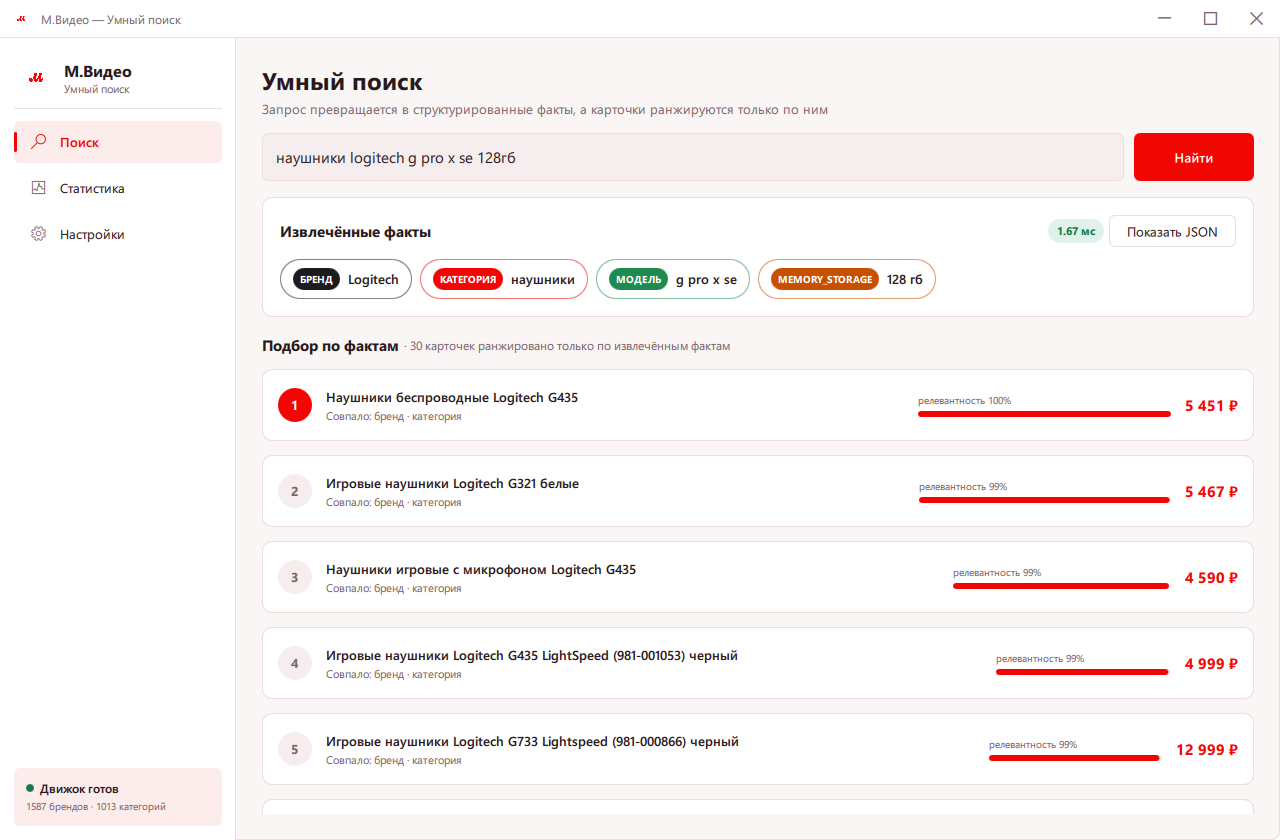
\includegraphics[width=0.98\textwidth,height=4.5cm,keepaspectratio]{cpp_mvp_search.png}
\par\vspace{3pt}
{\InterSemi\fontsize{8}{10}\selectfont Умный поиск}\par
{\smalltext\color{mvgray} Qt: факты чипами + выдача по извлечённым полям}
\column{0.48\textwidth}
\centering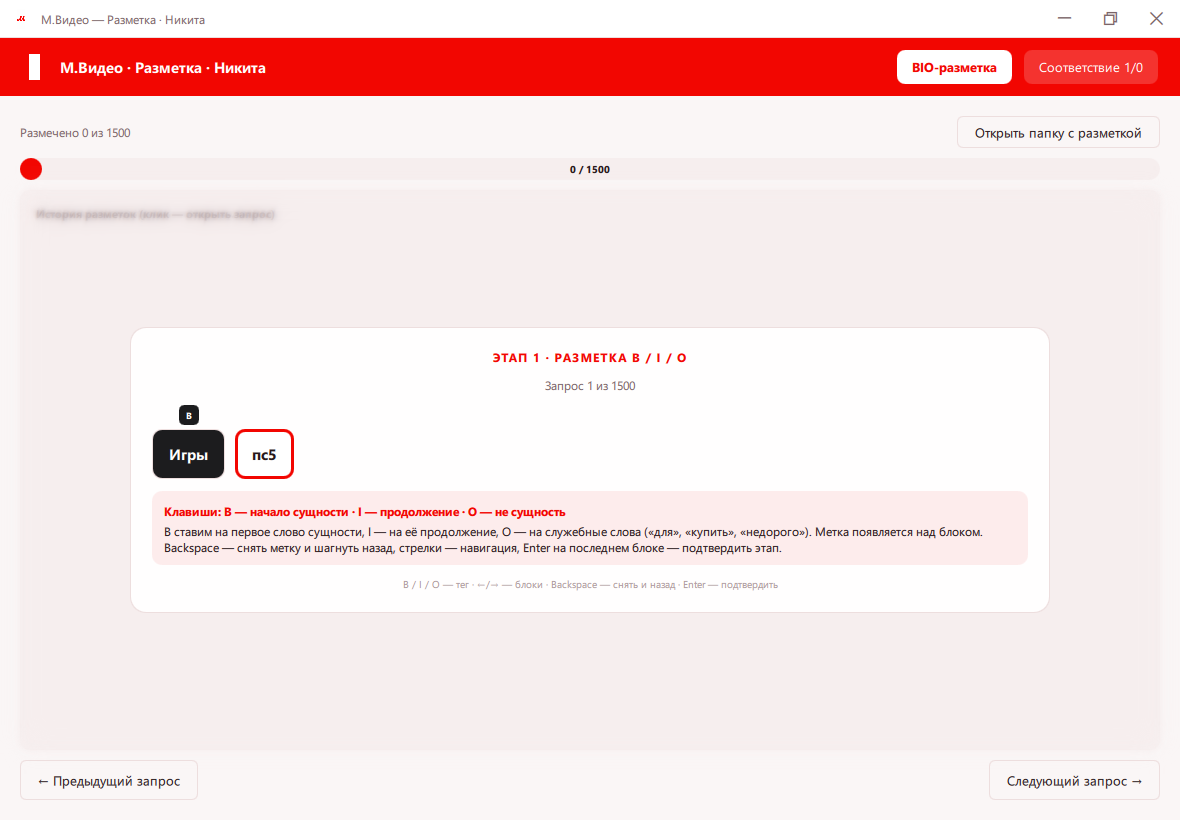
\includegraphics[width=0.98\textwidth,height=4.5cm,keepaspectratio]{cpp_label_stage1.png}
\par\vspace{3pt}
{\InterSemi\fontsize{8}{10}\selectfont Разметка}\par
{\smalltext\color{mvgray} BIO-мастер (B/I/O) + типы сущностей для золота}
\end{columns}
\slidefoot
\end{frame}

% ============================================================
% 17. ФИНАЛ
% ============================================================
\begin{frame}[plain]
\begin{tikzpicture}[remember picture, overlay]
  \fill[mvred] (current page.south west) rectangle (current page.north east);
  \node[anchor=east, inner sep=0pt] at ([xshift=0.32\paperwidth]current page.east)
    {
\includegraphics[height=1.06\paperheight]{kurs1_image1.png}};
  \node[anchor=west, align=left] at ([xshift=0.9cm, yshift=2.1cm]current page.west)
    {\color{white}\InterBold\fontsize{23}{27}\selectfont Спасибо!};
  \node[anchor=west, align=left, text width=0.52\paperwidth] at ([xshift=0.9cm, yshift=1.05cm]current page.west)
    {\color{white}\fontsize{9.5}{13}\selectfont Вопросы по пайплайну, SpellFix, GLiNER и метрикам — welcome.};
  \node[anchor=west, align=left, text width=0.55\paperwidth] at ([xshift=0.9cm, yshift=-0.85cm]current page.west)
    {\color{white}\fontsize{8.5}{13}\selectfont
     {\InterSemi Команда:}\\[2pt]
     Новицкий Никита · @n.novitskiy\\
     Борисов Никита · @n.borisov\\
     Засухина Елизавета · @e.zasukhina\\
     Олейников Александр · @a.oleynikov};
  \node[anchor=south west] at ([xshift=0.9cm, yshift=0.5cm]current page.south west)
    {\color{white}\fontsize{8}{10}\selectfont Презентация свёрстана в \TeX\ / \LaTeX\ · Итоги · Буткемп М.Видео};
\end{tikzpicture}
\end{frame}

\end{document}
